\documentclass{article}

\usepackage[left=2cm,right=2cm, top=2cm, bottom = 2cm]{geometry}
\usepackage{amsfonts}
%%%\usepackage{array}

\usepackage{amsmath}
\usepackage{xcolor}

\usepackage{tikz}
\usepackage{subfigure}

\pagestyle{empty}

\setlength{\tabcolsep}{15pt}
%%%\renewcommand{\arraystretch}{2.5}

%%%\makeatletter
%%%\newcommand{\thickhline}{%
%%%    \noalign {\ifnum 0=`}\fi \hrule height 2pt
%%%    \futurelet \reserved@a \@xhline
%%%}
%%%\newcolumntype{!}{@{\hskip\tabcolsep\vrule width 2pt\hskip\tabcolsep}}
%%%\makeatother

\newcommand{\deriv}[3][]{\frac{\mathrm{d}^{#1} #2}{\mathrm{d}#3^{#1}}}




\begin{document}

\title{Taylor Polynomials}
\date{}

\maketitle
\thispagestyle{empty}

\Large

\textbf{\underline{Objective: To understand how to approximate a differentiable}}

\textbf{\underline{function by polynomials about a point.}}




\vspace{5mm}


\textbf{Recap: The Newton-Raphson Method:}

\vspace{5mm}


Solve the equation $e^{-x}=\sin(x)$ to 3 significant figures, using a starting value of $x_1=1$.

\bigskip




\clearpage


{\bf Warm-Up: Determining Polynomials by Derivatives:}

\vspace{5mm}

\begin{enumerate}
	\item Find the unique straight line passing through $(0,2)$ with derivative $-7$, by the following steps:
		\begin{enumerate}
			\item Let the equation of the line be $y=mx+c$. Then we can find $\deriv{y}{x}$ and set it equal to $-7$ to find $m$.
			\item Substitute $x=0$, $y=2$ into the equation, since the line passes through $(0,2)$, to find $c$.
		\end{enumerate}
	\item Find the unique parabola ($y=ax^2+bx+c$) passing through $(0,2)$ with derivative $-7$ and second derivative $4$ at $x=0$ . Hint: adapt the strategy from question 1.
	\item Find the unique cubic curve passing through $(0,2)$ with derivative $-7$, second derivative $4$, and third derivative $1$ at $x=0$.
\end{enumerate}







\clearpage



\textbf{Theory: Taylor Polynomials:}

\vspace{5mm}

Polynomials are well-behaved and well-understood functions. As such, it can be useful to approximate more complicated functions by polynomials. Suppose we want to study the function $f(x)=e^x$ near $x=0$.\bigskip

Find the tangent to $y=f(x)$ at $x=0$ (the unique line passing through the same point, with the same gradient).

\vfill


Find the unique quadratic passing through the same point with the same first and second derivatives as $f(x)$ when $x=0$.


\vfill


Generalise this; find the unique degree-$n$ polynomial passing through the same point with the same first $n$ derivatives as $f(x)$ when $x=0$.

\vfill


Graphs are shown overleaf.


\clearpage






\textbf{Theory: Taylor Polynomials (cont.):}

\vspace{5mm}



\begin{figure}[h]
\centering

\subfigure{
	\begin{tikzpicture}[scale=0.5]
		\draw[->] (-6,0) -- (6,0);
		\draw[->] (0,0) -- (0,8);
		\node[right] at (6,0) {$x$};
		\node[above] at (0,8) {$y$};
		
		\draw[blue, thick, domain=-6:6,samples=100] plot (\x, {e^(\x/3)});
		
		\draw[red,thick,domain=-3:6,samples=100] plot (\x, {1+(\x/3)});
		

		\node[below] at (current bounding box.south) {$n=1$};
	\end{tikzpicture}
}
\subfigure{
	\begin{tikzpicture}[scale=0.5]
		\draw[->] (-6,0) -- (6,0);
		\draw[->] (0,0) -- (0,8);
		\node[right] at (6,0) {$x$};
		\node[above] at (0,8) {$y$};
		
		\draw[blue, thick, domain=-6:6,samples=100] plot (\x, {e^(\x/3)});
		
		\draw[red,thick,domain=-6:6,samples=100] plot (\x, {1+(\x/3)+0.5*(\x/3)^2});
		

		\node[below] at (current bounding box.south) {$n=2$};
	\end{tikzpicture}
}
	
\subfigure{
	\begin{tikzpicture}[scale=0.5]
		\draw[->] (-6,0) -- (6,0);
		\draw[->] (0,0) -- (0,8);
		\node[right] at (6,0) {$x$};
		\node[above] at (0,8) {$y$};
		
		\draw[blue, thick, domain=-6:6,samples=100] plot (\x, {e^(\x/3)});
		
		\draw[red,thick,domain=-6:6,samples=100] plot (\x, {1+(\x/3)+0.5*(\x/3)^2+(1/6)*(\x/3)^3});
		

		\node[below] at (current bounding box.south) {$n=3$};
	\end{tikzpicture}
}
\subfigure{
	\begin{tikzpicture}[scale=0.5]
		\draw[->] (-6,0) -- (6,0);
		\draw[->] (0,0) -- (0,8);
		\node[right] at (6,0) {$x$};
		\node[above] at (0,8) {$y$};
		
		\draw[blue, thick, domain=-6:6,samples=100] plot (\x, {e^(\x/3)});
		
		\draw[red,thick,domain=-6:6,samples=100] plot (\x, {1+(\x/3)+0.5*(\x/3)^2+(1/6)*(\x/3)^3+(1/24)*(\x/3)^4});
		

		\node[below] at (current bounding box.south) {$n=4$};
	\end{tikzpicture}
}
\caption{The graph of $y=e^x$ and its degree $n$ Taylor polynomials, for $n=1$, 2, 3, 4.}

\end{figure}


\vspace{1mm}

Let $f(x)$ be an $n$-times differentiable function. We define the \textbf{Taylor polynomial of degree $n$} of $f(x)$ around $x=a$ to be the unique polynomial of degree at most $n$ passing through the same point as $y=f(x)$ when $x=a$, and having the same first through to $n^\mathrm{th}$ derivatives at that point.\bigskip


Find the $n^\mathrm{th}$ Taylor polynomial of $f(x)$ about $x=a$.


\vfill



Rewrite this by changing variables to $h=x-a$.

\vfill






\clearpage

\textbf{Practice:}


\begin{enumerate}
	\item Compute the degree-8 Taylor polynomial of $\cos(x)$ about $x=0$. Graphs are shown overleaf.
	\item Compute the degree-8 Taylor polynomial of $\sin(x)$ about $x=0$.
	\item Compute the degree-3 Taylor polynomial of $\log_e(x)$ about $x=1$. Express this in the form $\log_e(1+x)=\hdots$
	\item Compute the degree-2 Taylor polynomial of $x^2e^{-x}$.
	\item \textbf{Difficult! Cautionary example:} Let $f(x)$ be the function defined by
		\[f(x)=\begin{cases}
				e^{-1/x^2} & :x\neq 0\\
				0 & :x=0
			\end{cases}\]
		Find the degree 1 Taylor polynomial of $f(x)$ about $x=0$ (you may assume that the derivative exists and is continuous at 0, so you can find the derivative for $x$ \textit{near} 0 and take the limit as $x\to 0$).\bigskip
		
		It can be shown that $f(x)$ is infinitely differentiable (can be differentiated as many times as you like), and all of its derivatives are 0 at $x=0$. Therefore every Taylor polynomial of $f(x)$ about $x=0$ is constantly 0. However, the function is non-zero everywhere except 0; so no matter how high a degree you take, the Taylor polynomial is never a good approximation away from $x=0$. The graph is shown below.
\end{enumerate}


\begin{center}
\begin{tikzpicture}
	\draw[->] (-6,0) -- (6,0);
	\node[right] at (6,0) {$x$};
	\draw[->] (0,0) -- (0,7);
	\node[above] at (0,7) {$y$};
	
	\draw[thick, red, domain=-6:6, samples=200] plot (\x, {6.5*2.718^(-1/(\x*\x/4))});
\end{tikzpicture}
\end{center}




\clearpage







\begin{figure}
\centering

\subfigure{
	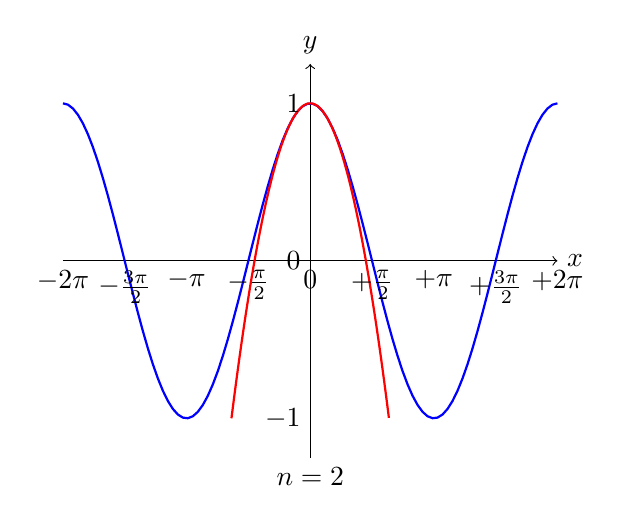
\begin{tikzpicture}[scale=0.5]
		\draw[->] (-6.28,0) -- (6.28,0);
		\draw[->] (0,-5) -- (0,5);
		\node[right] at (6.28,0) {$x$};
		\node[above] at (0,5) {$y$};
		
		\draw[blue, thick, domain=-6.28:6.28,samples=100] plot (\x, {4*cos(\x r)});
		
		\draw[red,thick,domain=-2:2,samples=100] plot (\x, {4*(1-(\x*\x)/2)});
		
		\foreach \i in {-1, 0, 1}{
			\node[left] at (0,4*\i) {$\i$};
		}
		
		\node[below] at (0,0) {$0$};
		\foreach \i in {+,-}{
			\node[below] at (\i 1.57,0) {$\i\frac{\pi}{2}$};
			\node[below] at (\i 3.14,0) {$\i\pi$};
			\node[below] at (\i 4.71,0) {$\i\frac{3\pi}{2}$};
			\node[below] at (\i6.28,0) {$\i2\pi$};
		}
		

		\node[below] at (current bounding box.south) {$n=2$};
	\end{tikzpicture}
}
\subfigure{
	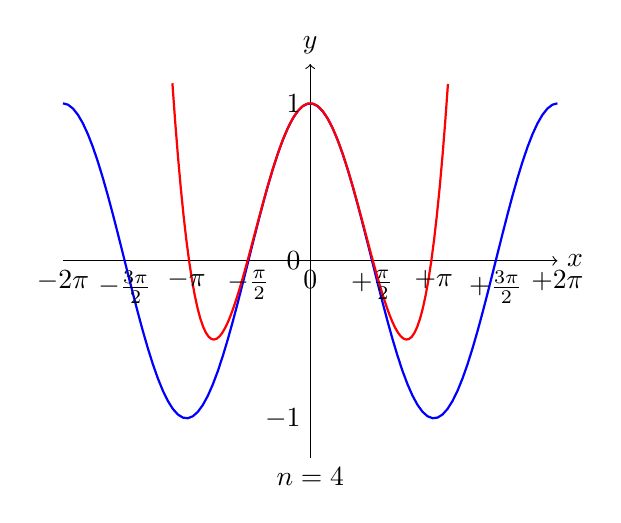
\begin{tikzpicture}[scale=0.5]
		\draw[->] (-6.28,0) -- (6.28,0);
		\draw[->] (0,-5) -- (0,5);
		\node[right] at (6.28,0) {$x$};
		\node[above] at (0,5) {$y$};
		
		\draw[blue, thick, domain=-6.28:6.28,samples=100] plot (\x, {4*cos(\x r)});
		
		\draw[red,thick,domain=-3.5:3.5,samples=100] plot (\x, {4*(1-(\x*\x)/2+(\x*\x*\x*\x)/24)});
		
		\foreach \i in {-1, 0, 1}{
			\node[left] at (0,4*\i) {$\i$};
		}
		
		\node[below] at (0,0) {$0$};
		\foreach \i in {+,-}{
			\node[below] at (\i 1.57,0) {$\i\frac{\pi}{2}$};
			\node[below] at (\i 3.14,0) {$\i\pi$};
			\node[below] at (\i 4.71,0) {$\i\frac{3\pi}{2}$};
			\node[below] at (\i6.28,0) {$\i2\pi$};
		}
		

		

		\node[below] at (current bounding box.south) {$n=4$};
	\end{tikzpicture}
}
	
\subfigure{
	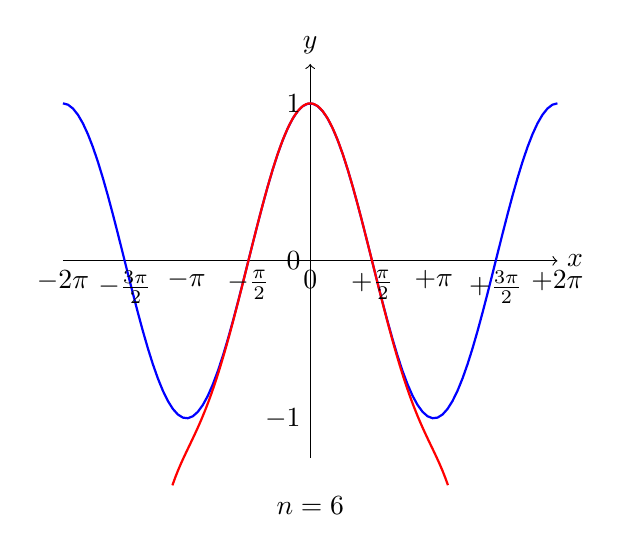
\begin{tikzpicture}[scale=0.5]
		\draw[->] (-6.28,0) -- (6.28,0);
		\draw[->] (0,-5) -- (0,5);
		\node[right] at (6.28,0) {$x$};
		\node[above] at (0,5) {$y$};
		
		\draw[blue, thick, domain=-6.28:6.28,samples=100] plot (\x, {4*cos(\x r)});

		\draw[red,thick,domain=-3.5:3.5,samples=100] plot (\x, {4*(1-(\x*\x)/2+(\x*\x*\x*\x)/24-(\x*\x*\x*\x*\x*\x)/720)});
		
		\foreach \i in {-1, 0, 1}{
			\node[left] at (0,4*\i) {$\i$};
		}
		
		\node[below] at (0,0) {$0$};
		\foreach \i in {+,-}{
			\node[below] at (\i 1.57,0) {$\i\frac{\pi}{2}$};
			\node[below] at (\i 3.14,0) {$\i\pi$};
			\node[below] at (\i 4.71,0) {$\i\frac{3\pi}{2}$};
			\node[below] at (\i6.28,0) {$\i2\pi$};
		}
		

		

		\node[below] at (current bounding box.south) {$n=6$};
	\end{tikzpicture}
}
\subfigure{
	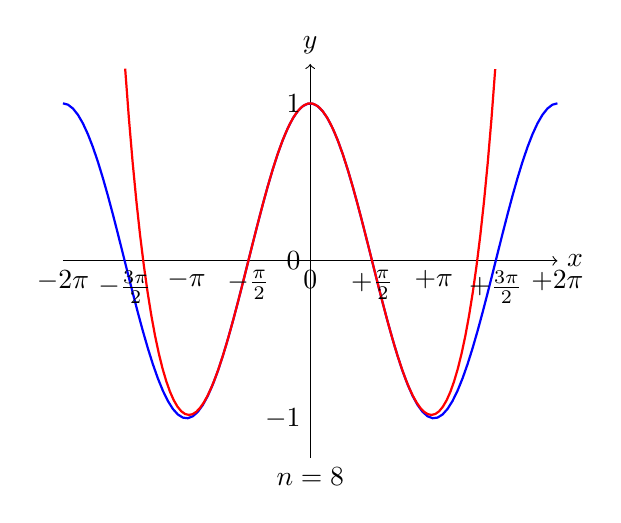
\begin{tikzpicture}[scale=0.5]
		\draw[->] (-6.28,0) -- (6.28,0);
		\draw[->] (0,-5) -- (0,5);
		\node[right] at (6.28,0) {$x$};
		\node[above] at (0,5) {$y$};
		
		\draw[blue, thick, domain=-6.28:6.28,samples=100] plot (\x, {4*cos(\x r)});
		
		\draw[red,thick,domain=-4.7:4.7,samples=100] plot (\x, {4*(1-(\x*\x)/2+(\x*\x*\x*\x)/24-(\x*\x*\x*\x*\x*\x)/720+((\x/8)*(\x/7)*(\x/6)*(\x/5)*(\x/4)*(\x/3)*(\x/2)*\x))});
		
		\foreach \i in {-1, 0, 1}{
			\node[left] at (0,4*\i) {$\i$};
		}
		
		\node[below] at (0,0) {$0$};
		\foreach \i in {+,-}{
			\node[below] at (\i 1.57,0) {$\i\frac{\pi}{2}$};
			\node[below] at (\i 3.14,0) {$\i\pi$};
			\node[below] at (\i 4.71,0) {$\i\frac{3\pi}{2}$};
			\node[below] at (\i6.28,0) {$\i2\pi$};
		}
		

		

		\node[below] at (current bounding box.south) {$n=8$};
	\end{tikzpicture}
}
\caption{The graph of $y=\cos(x)$, together with its degree-$n$ Taylor polynomials for $n=2$, 4, 6, and 8.}


\end{figure}

\vspace{3mm}

Note: In the Newton-Raphson method, we take the tangent to $y=f(x)$ at a point $x_n$, and find the point where that tangent hits the $x$-axis to be $x_{n+1}$. That tangent is precisely the degree 1 Taylor polynomial, $f_1(x)$, about $x=x_n$; so in fact the Newton-Raphson method consists of approximating a function by its degree one Taylor polynomial and then solving $f_1(x)=0$ to get an estimate for the solution of $f(x)=0$---and then of course iteratively using that estimate as the base point to find a new degree 1 Taylor polynomial, and repeat with that.

We could consider using higher degree Taylor polynomials in a Newton-Raphson-type method; for instance, we could take the degree 2 Taylor polynomial about $x_n$ and solve $f_2(x)=0$ to find a more accurate $x_{n+1}$; the problem with this is that quadratics have two roots, so $f_2(x)=0$ will give us two solutions, one of which is likely to be closer to the root of $f(x)$ than we would have got using $f_1(x)$, but the other of which could be anywhere. So we stick to using the degree 1 Taylor polynomial for Newton-Raphson and similar methods.


\clearpage
















{\bf Key Points to Remember:}

\vspace{5mm}

\begin{enumerate}
	\item A polynomial of degree $n$ can be entirely determined by specifying the value of the polynomial and its first $n$ derivatives at a single point.
	\item Given any $n$-times differentiable function $f(x)$, the \textbf{Taylor polynomial of degree $n$} of $f(x)$ about $x=a$ is $f_n(x)$, the unique polynomial of degree $n$ specified by the value and first $n$ derivatives of $f(x)$ at $x=a$. It is given by
		\begin{align*}
			f_n(x)&=f(a)+f'(a)(x-a)+\frac{f''(a)}{2!}(x-a)^2+ \hdots +\frac{f^{(n)}(a)}{n!}(x-a)^n\\
			&=\sum_{i=0}^n \frac{f^{(i)}(a)}{i!}(x-a)^i
		\end{align*}
		or
		\begin{align*}
			f_n(a+h)&=f(a)+f'(a)(h)+\frac{f''(a)}{2!}h^2 + \hdots +\frac{f^{(n)}(a)}{n!}h^n\\
			&=\sum_{i=0}^n \frac{f^{(i)}(a)}{i!}h^i.
		\end{align*}
	\item For values of $x$ close to $a$ (\textit{i.e.}, values of $h$ close to 0), the Taylor polynomial is typically a good approximation to the starting function: $f_n(x)\approx f(x)$. The higher the degree $n$, the further you can go from $a$ and maintain a good approximation. However, how good the approximation is at a certain distance from $a$ and for a given $n$ can vary a lot from function to function.
	\item For some functions, the Taylor polynomial fails to give a good approximation once you go too far from $a$, no matter how high a degree you take.
\end{enumerate}









\end{document}